% http://www.ctan.org/tex-archive/macros/latex/contrib/beamer/examples
% http://latex.artikel-namsu.de/english/beamer-examples.html

%\documentclass{beamer}
\documentclass[usenames,dvipsnames]{beamer}
\usepackage{amsmath}
\usepackage{amssymb}
\usepackage{bm}
\usepackage{fancybox, graphicx}
\usepackage{listings}
\usepackage{tikz} % Diagrams
\usepackage{color}
\usepackage{textcomp} % See https://tex.stackexchange.com/questions/145416/how-to-have-straight-single-quotes-in-lstlistings
\usepackage{multicol}
\usepackage{caption}

\lstset{language=bash,upquote=true} % Format listings as appropriate for bash. Inexplicably we get problems if the language is set as part of the \begin{lstlisting} command.

% https://tex.stackexchange.com/questions/36030/how-to-make-a-single-word-look-as-some-code
\definecolor{light-gray}{gray}{0.95}
\newcommand{\code}[1]{\colorbox{light-gray}{\texttt{#1}}}



\usetheme{boxes}
\usecolortheme{beaver}


\title{Introduction to High Performance Computing with GPUs}
\author{Lorne Whiteway \\ lorne.whiteway@star.ucl.ac.uk}
\institute{Astrophysics Group \\ Department of Physics and Astronomy \\ University College London}
\date{August 2018}

\subject{IT}

\begin{document}

\frame{\titlepage}


\begin{frame}{Where to find this presentation}
  \begin{block}{}
    Find the presentation at \alert{\url{https://tinyurl.com/yckg9mqa}}.\\
  \end{block}
  \begin{block}{}
    On this page click on `Download' to get a copy of the presentation.
  \end{block}
\end{frame}

\begin{frame}{Motivation}
  \begin{block}{}
    \begin{itemize}
      \item{Based in part on material from the course \textit{CUDA Programming on NVIDIA GPUs} by Mike Giles, Oxford.\\~\
      \url{http://people.maths.ox.ac.uk/~gilesm/cuda/}}\\~\
      \item{Opinions expressed are my own...}
    \end{itemize}
  \end{block}
\end{frame}

\begin{frame}{Two paradigms}
  \begin{block}{}
    \begin{itemize}
      \item{Intel (market cap \$220B\footnotemark): One-chip-fits-all. Use the same chip (a CPU) for all tasks e.g. both word processing and high-performance computing (HPC).}\\~\
      \item{NVIDIA (market cap \$152B\footnotemark[\value{footnote}]): Create a specialised chip (the GPU) specifically tailored for certain tasks (including HPC).}
    \end{itemize}
  \end{block}
  \footnotetext[\value{footnote}]{As of 27 July 2018}
\end{frame}

\begin{frame}{GPUs}
  \begin{block}{}
    \begin{itemize}
      \item{GPU  = graphics processing unit}
      \item{Specialised chip}
      \item{Has many processors and a specialised memory structure}
      \item{Originally designed specifically for high performance via parallelisation when doing graphics rendering.}
      \item{Single instruction, multiple data (SIMD).}
      \item{This design also makes them suitable for parallelizable problems in HPC.}
      \item{Not-standalone - needs a CPU `host'.}
    \end{itemize}
  \end{block}
\end{frame}

\begin{frame}{GPU \tiny{Image credit: NVIDIA \url{https://www.nvidia.com/en-us/data-center/tesla-v100/}}}
  \begin{block}{}
    \begin{center}
      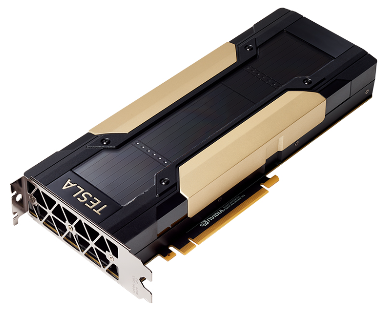
\includegraphics[scale=0.83]{V100_photo.png}
    \end{center}
  \end{block}
\end{frame}

\begin{frame}{GPUs are displacing CPUs for HPC}
  \begin{block}{}
    \begin{itemize}
      \item{GPUs offer better value (FLOPS/\$) and energy usage (FLOPS/J) than CPUs.}\\~\
      \item{5 of the world's top 7 supercomputers use GPUs, including the top supercomputer (\textit{Summit}, Oak Ridge National Lab, 122.3 PFLOPS).\footnotemark}\\~\
      \item{All else being equal, we should probably use GPUs for HPC...}
    \end{itemize}
  \end{block}
\footnotetext[\value{footnote}]{TOP500 list, June 2018 \url{https://www.top500.org/lists/2018/06/}}
\end{frame}

\begin{frame}{But...}
  \begin{block}{}
    \begin{itemize}
      \item{Installed base of CPUs (e.g. splinter).}\\~\
      \item{Takes time to develop GPU expertise.}\\~\
      \item{Program code needs to be altered to run (effectively) on GPUs.}
    \end{itemize}
  \end{block}
\end{frame}

\begin{frame}{GPUs on splinter}
  \begin{block}{}
    \begin{itemize}
      \item{New (July 2018) GPU `Tesla V100' (in addition to old `K80').}\\~\
      \item{Thanks to Ofer (funding) and Edd (implementation)!}\\~\
      \item{How can we use these cards effectively?}
    \end{itemize}
  \end{block}
  \begin{figure}
  \begin{multicols}{2}
  \centering
  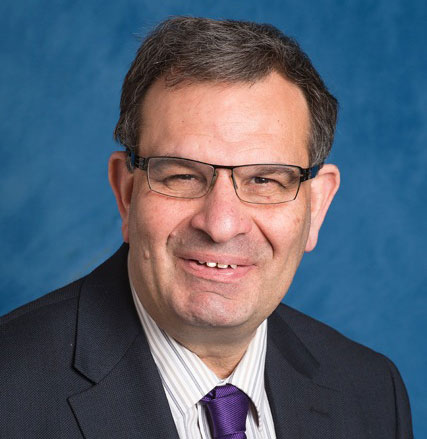
\includegraphics[width=0.18\textwidth]{Ofer_Lahav_photo_2014_SB_STFC.jpg}\\
  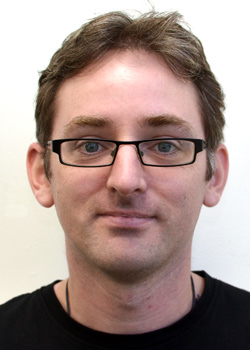
\includegraphics[width=0.13\textwidth]{Edward_Edmonson_2016_w.jpg}\\
  \end{multicols}
  \end{figure}
\end{frame}

\begin{frame}{Tesla V100 specifications} {\tiny Image credit: NVIDIA \url{http://www.nvidia.com/content/PDF/Volta-Datasheet.pdf}}
  \begin{block}{}
    \begin{center}
      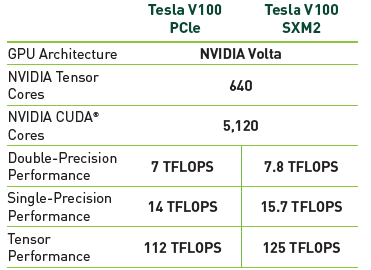
\includegraphics[scale=0.90]{V100_specsheet_A.png}
    \end{center}
  \end{block}
\end{frame}

\begin{frame}{Tesla V100 specifications} {\tiny Image credit: NVIDIA \url{http://www.nvidia.com/content/PDF/Volta-Datasheet.pdf}}
  \begin{block}{}
    \begin{center}
      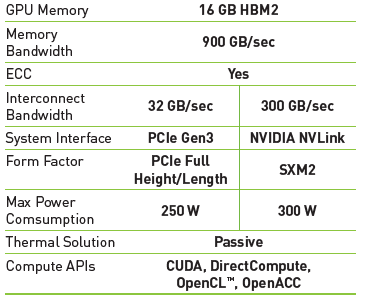
\includegraphics[scale=0.83]{V100_specsheet_B.png}
    \end{center}
  \end{block}
\end{frame}

\begin{frame}{Next problem...}
  \begin{block}{}
    \begin{itemize}
      \item{When you solve your biggest problem you simply get a new biggest problem.}\\~\
      \item{Large number of processors should slash computation wallclock time for parallelizable problems.}\\~\
      \item{But in fact we simply discover that speed of memory read/write becomes the new bottleneck.}\\~\
    \end{itemize}
  \end{block}
\end{frame}

\begin{frame}{GPU memory hierarchy}
  \begin{block}{}
    \begin{itemize}
      \item{GPUs have a \textit{memory hierarchy} (moving down the list: faster, smaller, more expensive):}
      \begin{itemize}
      \item{CPU (`host') core memory}
      \item{GPU (`device') core memory}
      \item{Level 2 (`L2') cache}
      \item{Level 1 (`L1') cache}
      \item{Registers}\\~\
      \end{itemize}
      \item{GPU-destined software must keep this hierarchy in mind.}\\~\
    \end{itemize}
  \end{block}
\end{frame}

\begin{frame}{CPU $\leftrightarrow$ GPU relatively slow}
  \begin{block}{}
    \begin{itemize}
      \item{Data transfer links as fast as possible. But e.g. CPU host $\leftrightarrow$ GPU device is relatively slow.}\\~\
      \item{Some problems are simply not worth doing on the GPU as it would be slower to copy the data to the GPU than it would be to do the calculation non-parallel on the CPU.}\\~\
      \item{Not worth copying a number to the GPU unless you are going to do roughly 100 FLOPS with it.}\\~\
      \item{But e.g. matrix multiplication is certainly worth doing on the GPU as copying data is $\mathcal{O}(N^2)$ while the calculation is $\mathcal{O}(N^3)$.}\\~\
    \end{itemize}
  \end{block}
\end{frame}

\begin{frame}{Parallel Programming - threads}
  \begin{block}{}
    \begin{itemize}
      \item{The code that runs on the GPU should create multiple threads; one thread will get attention from one processor.}\\~\
      \item{Generally you want many, many threads at the same time (to keep all the processors busy); if the problem is parallelizable then you should be able to organise the code to achieve this (e.g. each thread deals with part of the data).}\\~\
      \item{The threads will get batched into sets of 32 threads called \textit{warps} and you want many such warps.}\\~\
    \end{itemize}
  \end{block}
\end{frame}

\begin{frame}{Parallel Programming - warps}
  \begin{block}{}
    \begin{itemize}
      \item{The 32 threads in a warp run in absolute lockstep - they all execute the same code at the same time on different data (SIMD).}\\~\
      \item{Consider\\~\ \texttt{threadID < 8 ? f(x) : g(x);}\\~\ \noindent here the first 8 threads calculate f while 24 threads twiddle their thumbs, \textbf{then} 24 threads calculate g while 8 threads twiddle their thumbs. Suboptimal.}
    \end{itemize}
  \end{block}
\end{frame}

\begin{frame}{GPU programming: CUDA}
  \begin{block}{}
    \begin{itemize}
      \item{CUDA is a language in which you can write code that will execute efficiently on a GPU.}\\~\
      \item{CUDA is \texttt{C}, plus templates, plus a few CUDA-specific language instructions. Use extention \texttt{.cu}.}\\~\
      \item{There is a CUDA compiler \texttt{nvcc} (I suspect that it's just a \texttt{C} preprocessor...)}\\~\
      \item{Can link with other C, C++, Fortran object files.}\\~\
    \end{itemize}
  \end{block}
\end{frame}

\begin{frame}{CUDA example - see handout}
  \begin{block}{}
    \begin{center}
      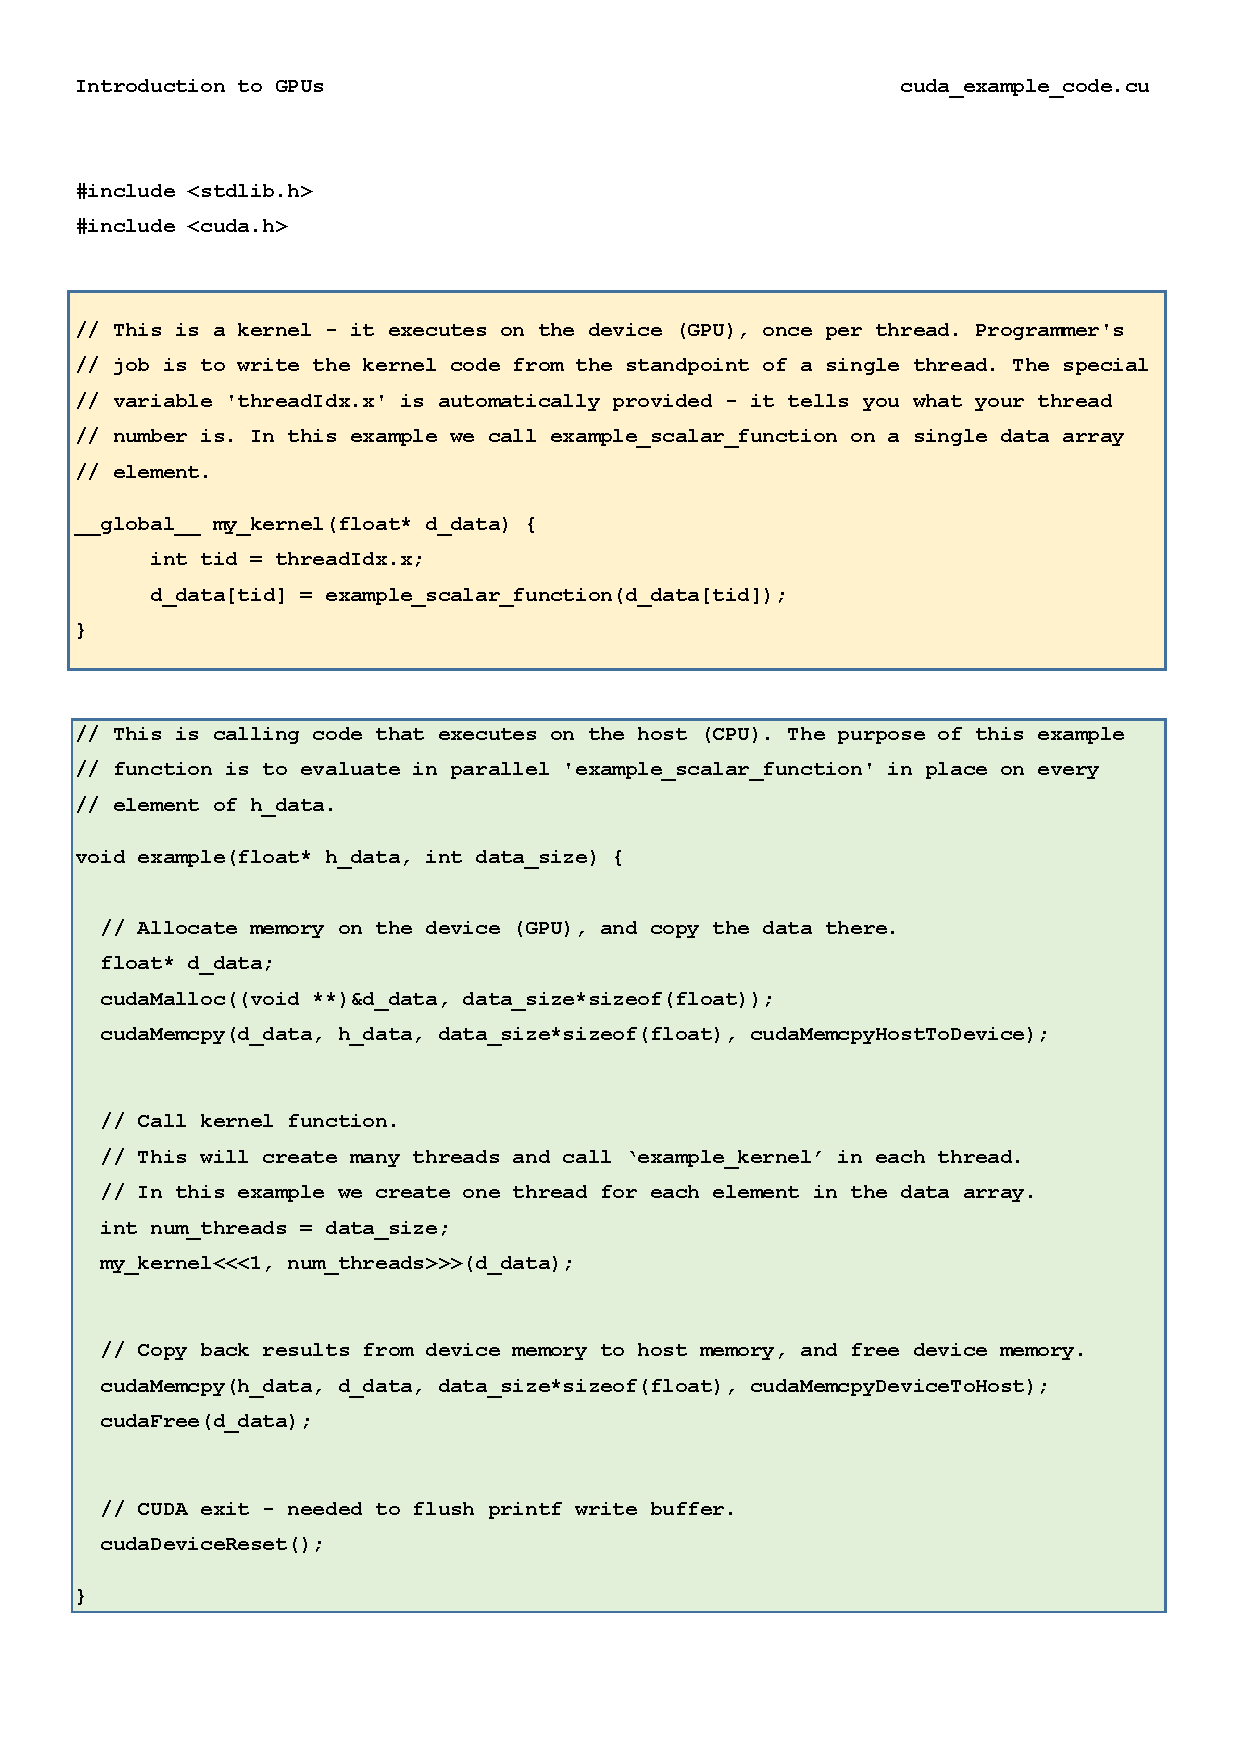
\includegraphics[scale=0.23]{cuda_example_code.pdf}
    \end{center}
  \end{block}
\end{frame}

\begin{frame}{CUDA example - host code (green)}
  \begin{block}{}
    \begin{itemize}
      \item{Need to copy data to device, so \texttt{malloc} then \texttt{memcpy}. But the host cannot see the device memory explicitly, so use special CUDA functions to do this.}\\~\
      \item{The `kernel' is the code that will run on the GPU. Special syntax $\langle\langle\langle \texttt{1, num\_threads} \rangle\rangle\rangle$ to specify number of threads; also has a normal argument list.}\\~\
    \end{itemize}
  \end{block}
\end{frame}

\begin{frame}{CUDA example - device code (yellow)}
  \begin{block}{}
    \begin{itemize}
      \item{Special keyword \texttt{\_\_global\_\_} identifies kernel function.}\\~\
      \item{Written from the point of view of one thread (like MPI, not like OpenMP).}\\~\
      \item{Special variable \texttt{threadIdx.x} automagically tells the kernel code what thread it is running in.}\\~\
    \end{itemize}
  \end{block}
\end{frame}

\begin{frame}{Organisation of threads}
  \begin{block}{}
    \begin{itemize}
      \item{32 threads in a warp - they move in absolute lockstep.}\\~\
      \item{Up to 32 warps in a \textit{block}. All the threads in a block can share some L1 cache memory.\footnotemark}\\~\
      \item{As many blocks as you want (running on one GPU). All threads in the GPU can share some L2 cache memory.}\\~\
      \item{There are also methods for running across multiple GPUs...}\\~\
    \end{itemize}
  \end{block}
\footnotetext{Maximum threads in a block depends on the GPU architecture}
\end{frame}

\begin{frame}{Organisation of threads}
  \begin{block}{}
    \begin{itemize}
      \item{Thus thread organisation is hierarchical (just as it was with memory organisation).}\\~\
      \item{This reflects a preference for `fine control at multiple levels' (in the persuit of maximum performance) at the cost of simplicity of design.}\\~\
    \end{itemize}
  \end{block}
\end{frame}

\begin{frame}{CUDA code with multiple thread blocks}
  \begin{block}{}
    \begin{itemize}
      \item{In the caller:\newline
      \texttt{int threads\_per\_block = 32;}\newline
      \texttt{int n\_blocks = data\_size / threads\_per\_block;}\newline
      \texttt{my\_kernel}$\langle\langle\langle$\texttt{n\_blocks, threads\_per\_block}$\rangle\rangle\rangle$\texttt{(d\_data);}
      }\\~\
      \item{In the kernel:\newline
      \texttt{int tid = threadIdx.x + blockDim.x * blockIdx.x}
      }
    \end{itemize}
  \end{block}
\end{frame}

\begin{frame}{Synchronisation}
  \begin{block}{}
    \begin{itemize}
      \item{Threads in a warp move in lockstep but otherwise no guarantees of synchronicity - thread 145 might finish before thread 13 begins.}
      \item{There are functions to implement synchronisation (across threads in a block, or across all blocks).}
      \item{Can set up some shared memory for all the threads in a block.}
      \item{There are some \textit{atomic} functions e.g. for modifying a global variable; your thread will briefly get a lock on the global variable.}
      \item{Very fast functions to allow threads in a warp to exchange information (warp shuffles).}
    \end{itemize}
  \end{block}
\end{frame}

\begin{frame}{Cache lines}
  \begin{block}{}
    \begin{itemize}
      \item{Data is read in a \textit{cache line} of 64 bytes (8 doubles) - if you ask for only one double, you will still get 8. Only a few cache lines can be held in fast memory at a time.}\\~\
      \item{You should already be taking this into account when programming CPUs. For example, it makes sense to process an array sequentially, so as not to `churn' the cache lines.}\\~\
      \item{Still an issue with GPUs, but here you need sensible interaction with the cache lines across \textit{all} the threads in a warp.}
    \end{itemize}
  \end{block}
\end{frame}

\begin{frame}{Single or double precision?}
  \begin{block}{}
    \begin{itemize}
      \item{Should you use single or double precision? GPUs support both, but there's a performance difference (of the factor that you would expect).}\\~\
      \item{Of course this is also a concern with CPUs.}\\~\
      \item{CUDA supports templates, so it's easy to experiment.}\\~\
      \item{GPU also supports half-precision data type.}
    \end{itemize}
  \end{block}
\end{frame}

\begin{frame}{Streams}
  \begin{block}{}
    \begin{itemize}
      \item{The GPU can transfer data into and out of memory at the same time as it is doing calculations.}\\~\
      \item{Thus it makes sense to organise the code so that both operations happen at the same time (on different data sets, obviously).}\\~\
      \item{\textit{Streams} are a CUDA construct to allow this.}
    \end{itemize}
  \end{block}
\end{frame}

\begin{frame}{Tuning}
  \begin{block}{}
    \begin{itemize}
      \item{The performance of an algorithm on a GPU often depends sensitively to CUDA parameters. (How many threads? How many threads per block? How many streams?)}\\~\
      \item{Can get e.g. ten-fold performance improvement with correct choice of parameters..}\\~\
      \item{Therefore crucial to experiment with different parameters.}
    \end{itemize}
  \end{block}
\end{frame}

\begin{frame}{Parallel algorithms - summation}
  \begin{block}{}
    \begin{itemize}
      \item{Summing N numbers can be done in $\log_2(N)$ (parallel) steps.\\~\
      In the first step, nodes 0 and 1 exchange data (so then each knows $x_0 + x_1$); simultaneously 2 and 3 exchange, 4 and 5 exchange, etc.\\~\
      In the second step, nodes 0 and 2 exchange subtotals (so then each knows $x_0 + x_1 + x_2 + x_3$), etc.;\\~\
      Etc.}\\~\
      \item{Warp shuffles make this easy and fast (at least for the first five steps).}\\~\
      \item{Similar logic used for the Fast Fourier Transform (FFT).}
    \end{itemize}
  \end{block}
\end{frame}

\begin{frame}{Parallel algorithms - other examples}
  \begin{block}{}
    \begin{itemize}
      \item{Many other problems (apparently sequential in nature) actually can be solved in parallel. How would you parallelise the following?}\\~\
      \begin{itemize}
        \item{Partial sumation (a.k.a. \textit{scan} operation): calculate $x_0, x_0+x_1, x_0+x_1+x_2, \ldots$\\~\ This plays a role in parallel sorting algorithms.}\\~\
        \item{Solve tridiagonal linear system.}\\~\
      \end{itemize}
      \item{The answers to these questions have been known for decades (parallel computation is not a new idea...)}
    \end{itemize}
  \end{block}
\end{frame}

\begin{frame}{Parallel algorithms - FFT}
  \begin{block}{}
    \begin{itemize}
      \item{CUDA makes a parallel FFT algorithm available; the interface to this is \texttt{C}, not CUDA. Thus your \texttt{C} or \texttt{C++} code can calculate FFT on GPUs without you needing to write CUDA code.}\\~\
      \item{There are two interfaces: one mimics the FFTW interface (for easy transition) while the other is `the right one'.}\\~\
    \end{itemize}
  \end{block}
\end{frame}

\begin{frame}{Interfaces}
  \begin{block}{}
    \begin{itemize}
      \item{Many users would probably be content to use interfaces that shielded them from the CUDA details (as with FFT).}\\~\
      \item{But the devil is in the detail; e.g. need some awareness of how CUDA works to ensure algorithm operates at peak efficency.}\\~\
      \item{CUDA FFT algorithm `self-tunes' its parameters when first installed on a new system.}
    \end{itemize}
  \end{block}
\end{frame}

\begin{frame}{CUDA ecosystem}
  \begin{block}{}
    \begin{itemize}
      \item{SDK with many examples.}\\~\
      \item{Good documentation (except perhaps for the compiler).}\\~\
      \item{Online community.}\\~\
      \item{\textit{Nsight}, a visual development environment (plug-in for Eclipse and Visual Studio).}\\~\
      \item{Excellent tools for debugging and for profiling.}
    \end{itemize}
  \end{block}
\end{frame}

\begin{frame}{Does CUDA have a long-term future?}
  \begin{block}{}
    \begin{itemize}
      \item{\texttt{C}, \texttt{C++} and \texttt{FORTRAN} have remained popular since they are close-to-ideal for abstractly expressing sequential algorithms. They have survived despite huge changes in computer architecture.}\\~\
      \item{Is CUDA similarly close-to-ideal for abstractly expressing parallel algorithms?.}\\~\
      \item{Or is it too tied up with peculiarities of the GPU card? Will CUDA code go out-of-date as hardware changes?}\\~\
      \item{Also, CUDA is a proprietary language; NVIDIA appears to be `nice' but its concerns are commercial ones.}
    \end{itemize}
  \end{block}
\end{frame}

\begin{frame}{CUDA alternatives}
  \begin{block}{}
    \begin{itemize}
      \item{\textit{OpenCL} is an open standard that competes with CUDA. Used for smartphone apps, but otherwise CUDA appears to be winning.}\\~\
      \item{\textit{Thrust} hides CUDA code behind a \texttt{C++} STL-like interface.}\\~\
      \item{\textit{Kokkos} is another \texttt{C++} template library for GPU code.}\\~\
      \item{\textit{OpenACC} appears to be an attempt to merge CUDA and OpenMP.}\\~\
      \item{Unclear which of these if any will win out.}
    \end{itemize}
  \end{block}
\end{frame}

\begin{frame}{Tensor cores}
  \begin{block}{}
    \begin{itemize}
      \item{Machine learing applications are commercially important enough for NDVIDIA to have built special processors (`tensor cores') onto the Tesla V100 card.}\\~\
      \item{These are optimised to perform matrix multiplications of 16-bit floats, but then accumulate the product as 32-bit doubles.}\\~\
      \item{This hardware can then be used by TensorFlow.}\\~\
      \item{NVIDIA will provide specialised hardware for your application only if you can guarantee billions of dollars of sales...}
    \end{itemize}
  \end{block}
\end{frame}

\begin{frame}{GPU users}
  \begin{block}{}
    \begin{itemize}
      \item{Gamers (and bitcoin miners, who have similar computational needs) are one category - the `GForce' card is aimed at them.}\\~\
      \item{Data centres and machine learning is another category - the `Tesla' card is aimed at them.}\\~\
      \item{Scientific HPC also uses `Tesla' technology. My impression is that NVIDIA takes this customer base seriously, not because of sales volumes, but to encourage R\&D exchange.}
    \end{itemize}
  \end{block}
\end{frame}

\begin{frame}{On the horizon}
  \begin{block}{}
    \begin{itemize}
      \item{Faster data exchange between GPUs.}\\~\
      \item{Direct flow of incoming real-time data onto the GPU; self-driving cars will do this.}\\~\
      \item{Both of these make the CPU less central.}
    \end{itemize}
  \end{block}
\end{frame}

\end{document}
